% !TEX root = main.tex

\section{EyeNav}

\begin{figure}[h]
	\centering
	\vspace{-10pt}
	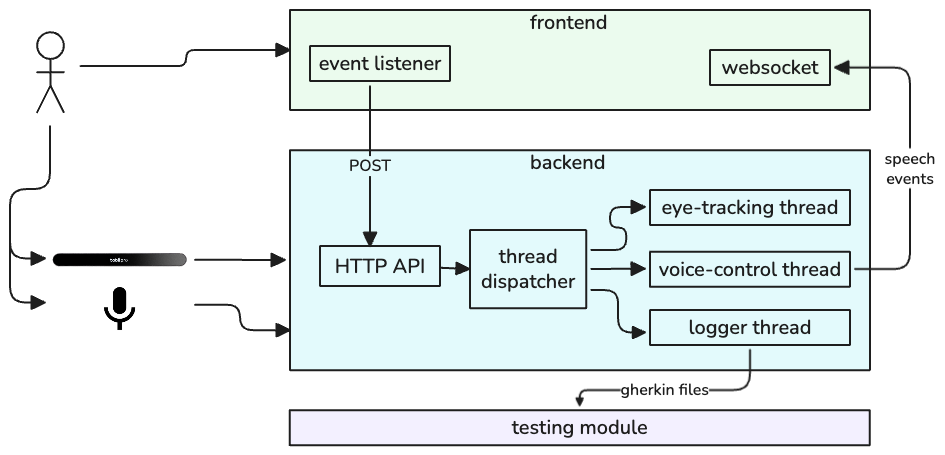
\includegraphics[width=180pt]{imgs/diagram-context.png}
	\caption{Context diagram of the system.}
	% \vspace{-10pt}
	\label{fig:context}
\end{figure}

This section outlines the EyeNav system based on its workflow, as illustrated in Fig.~\ref{fig:context}. EyeNav is composed of 2 main modules: (i) a Chrome Extension sidebar and (ii) a backend module built in python. The Chrome extension sidebar, which functions as an adjacent webpage alongside the main content, presents the available verbal commands, allows to initiate a interaction session, and shows the interpreted verbal commans in realtime once a session has started (See Fig.~\ref{fig:requirements}). Once a session begins, the system orchestrates multiple components, including voice recognition, eye tracking, and interaction logging.

\begin{figure}[h]
	\centering
	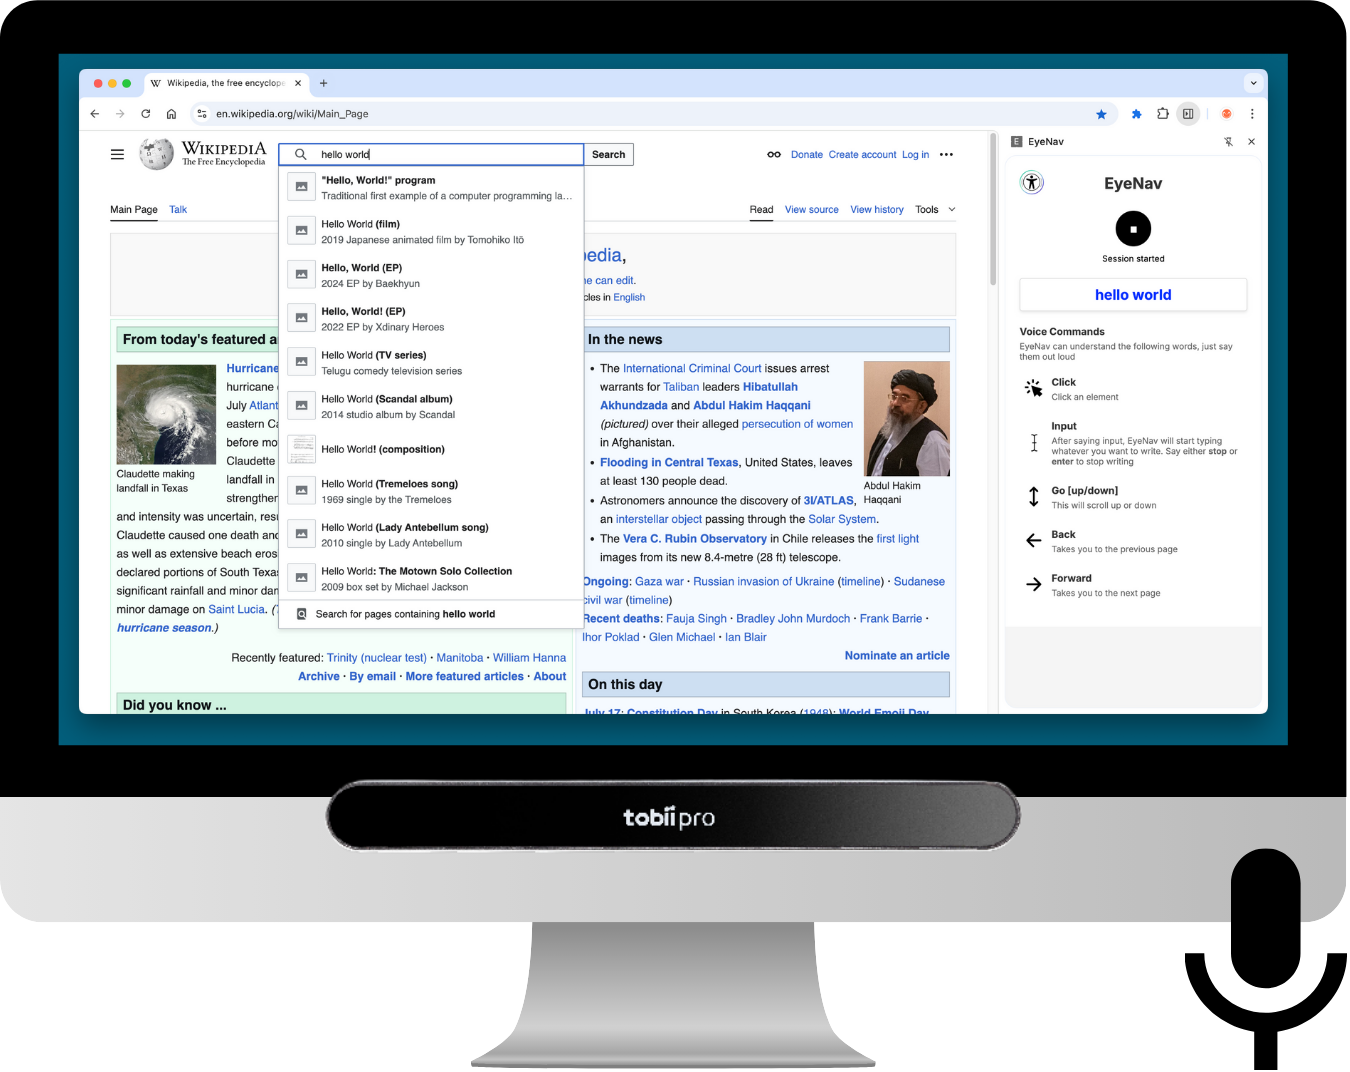
\includegraphics[width=180pt]{imgs/system-requirements.png}
	\caption{A graphic of what the system looks like}
	% \vspace{-13pt}
	\label{fig:requirements}
\end{figure}

User input is captured via an eye-tracker and microphone, while the underlying processing occurs in a backend service rather than on the frontend. Concurrently, user interactions, such as clicks, text input, and navigation events, are recorded by a logging module. These events are compiled into an executable test file, which can later be replayed using Gherkin-based test execution tools like Selenium\cite{garcia2024selenium} or Kraken\cite{ravelo2023kraken}.


\subsection{High-Level Architecture}

\begin{figure}
    \centering
    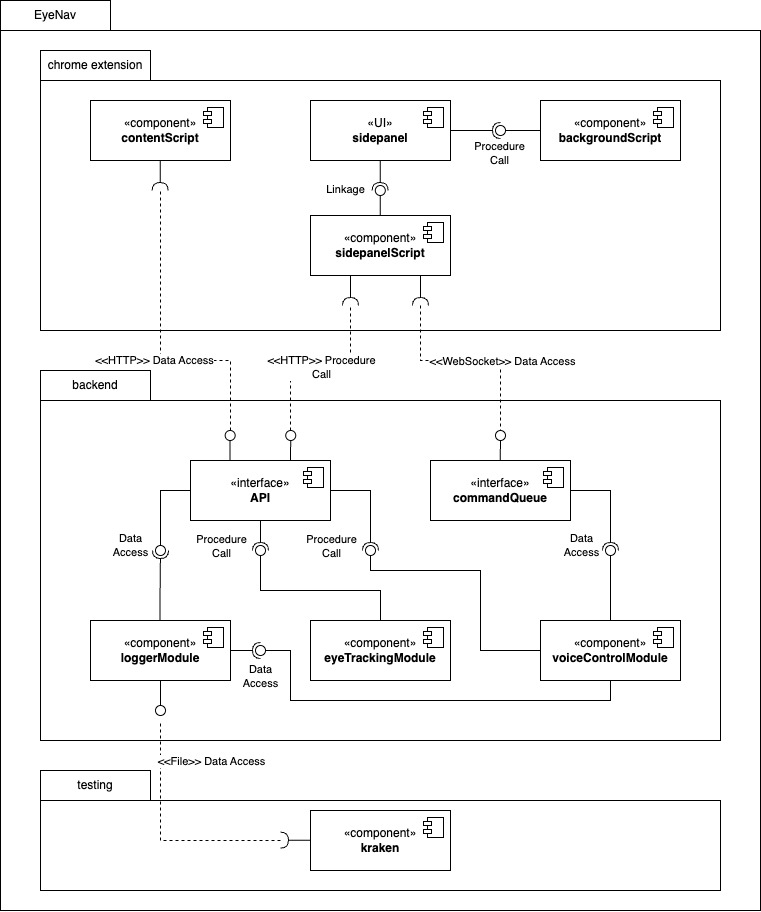
\includegraphics[width=200pt]{imgs/components-diagram.jpg}
    \caption{Components diagram}
    \vspace{-13pt}
    \label{fig:components-diagram}
\end{figure}

Figure ~\ref{fig:components-diagram} presents the complete component architecture of the system.

The Chrome extension serves as the front-end interface, providing real-time textual feedback for recognized voice commands and capturing user interaction events. Click events are detected on the frontend and forwarded as HTTP POST requests to the backend to preserve contextual information, such as the associated HTML tag. 

Eye tracking is powered by the Tobii Pro Nano, a single-camera dark/bright pupil system with corneal reflection and a typical latency of approximately 17 ms~\cite{tobiiabndpronano}. The gaze-driven pointer control module uses the \verb|tobii-research| Python SDK to access real-time gaze data and interpolate cursor movement accordingly.

Voice commands are captured through a microphone and transcribed using the Vosk speech recognition engine\cite{vosk2025}, which operates entirely on-device for privacy and low latency. Recognized phrases are matched to predefined command templates and sent to the backend over WebSocket connections, enabling minimal response delay.

The backend integrates data from both the Tobii eye-tracker and the Vosk engine to interpret user intent, translate inputs into executable UI commands, and log all interactions. These are executed using Kraken, a behavior-driven testing framework built on WebdriverIO\cite{webdriverio}, supporting usability and regression testing even under dynamic UI conditions.

The system is organized into modular components, each adhering to a single-responsibility design principle. These include: (1) the gaze-driven pointer control, which enables real-time cursor positioning based on eye movement; (2) the NLP-based command parsing module, which interprets speech input captured by Vosk and maps it to specific UI actions among clicks, text entry, and scrolling; and (3) the record-and-replay test generation module, which logs user interactions in Gherkin syntax and compiles them into executable test scripts compatible with WebdriverIO for automated testing.

\section{EyeNav Capabilities}
\subsection{Voice Commands}

The current implementation supports four voice commands: \textit{Click}, \textit{Input}, \textit{Go (up/down)}, and \textit{Navigate (back/forward)}. These commands were selected to reflect fundamental browser interactions typically performed via mouse and keyboard, providing a minimal yet functional command set suitable for a prototype. Each command corresponds to a distinct action: Click triggers a mouse click, Input captures and types dictated speech, Go scrolls the page vertically in the specified direction, and Navigate back or forward transitions between last and next pages in the browser history.

\subsection{NLP in multiple languages}
Accessibility also encompasses internationalization, and the system is designed to adapt to the user's preferred browser language. Currently, it supports both English and Spanish, with additional languages easily integrable by downloading the corresponding voice recognition model and translating the interface localization files.

\subsection{Test Case generation}

Interaction logging follows a structured hierarchy for element identification. For click events, the Chrome extension attaches a global event listener to the entire page, maintained dynamically via a \verb|MutationObserver| to accommodate changes in the DOM. Only interactions with semantically clickable elements, including hyperlinks, buttons, and similar controls, are considered. When such an element is clicked, the system attempts to identify it using a prioritized attribute hierarchy: \verb|href|, \verb|id|, \verb|className|, and, if necessary, an automatically computed \verb|xPath|. This hierarchical strategy ensures that the most stable and descriptive selector available is used for referencing the element in the generated test script.


\begin{lstlisting}
Feature: Replay of session on MM DD at HH:MM:SS [AM/PM]

@user1 @web
Scenario: User interacts with the web page named "Amazon.com. Spend less. Smile more."

	Given I navigate to page "https://www.amazon.com/"
	And I click on tag with id "twotabsearchtextbox"
	And I input "nike black shoes"
	And I click on tag with id "nav-search-submit-button"
	And I scroll down
	And I click on tag with xpath "/html[1]/body[1]/div[1]/div[1]/div[1]/div[1]/div[1]/span[1]/div[1]/div[9]/div[1]/div[1]/span[1]/div[1]/div[1]/div[1]/span[1]/a[1]/div[1]"
\end{lstlisting}

The latter is an example of a generated test file. Each instruction is written in Gherkin syntax, promoting both human readability and maintainability. This format is particularly accessible to non-technical stakeholders while remaining fully compatible with the automated testing frameworks employed in the system.

\subsection{Accessible Interaction}
EyeNav supports keyboard navigation via the Tab key, enabling users to traverse interactive elements.

\section{EyeNav Use Cases}

Since each component operates independently, this flexibility allows the system to support a variety of use cases, each leveraging different capabilities of the tool.

\subsection{Accessible Interaction Mechanism for Web Applications}
Users with motor impairments or those seeking hands-free control can benefit from the gaze-based and voice-driven interface, offering an accessible and intuitive method of web navigation without the need for traditional input devices.

\subsection{Record-and-Replay Testing Tool (A-TDD)}

The logger module functions independently of the input modality, meaning it can be used even with conventional mouse and keyboard input. As such, EyeNav also serves as a lightweight, behavior-driven development (BDD) tool suitable for acceptance test-driven development (A-TDD) workflows.

\subsection{Support for Accessibility Evaluation Professionals}

The system provides a valuable platform for accessibility consultants, QA engineers, and researchers conducting accessibility evaluations. Its support for multimodal input—via eye tracking, voice recognition, or a combination of both—enables flexible testing setups tailored to a wide range of users and scenarios, including those that simulate real-world accessibility constraints.

\subsection{Intelligent Agents and Automation Scenarios}

EyeNav's architecture allows for the integration of intelligent agents capable of interpreting and executing multimodal input. In envisioned scenarios, agents powered by NLP models could use EyeNav to autonomously interact, also using speech or other simulated modalities, with web interfaces. These interactions can also be recorded using the logger module, enabling automated usability assessments and supporting research in autonomous accessibility testing.

\section{Results}

\subsection{User Feedback}

Qualitative interviews identified several key usability factors. Larger UI elements significantly improved gaze accuracy, making it easier for users to select targets with their eyes. Voice commands were most effective when they were short and distinct, reducing recognition errors. Environmental noise was found to negatively impact the reliability of speech recognition, suggesting the need for robust filtering or alternative input strategies. Users also indicated that visual indicators for "gaze hover targets" would enhance feedback and confidence during interaction. Additionally, simplified scroll commands were perceived as more usable and intuitive compared to earlier, more granular versions.

\subsection{Accessibility Insights}

Testers noted that this input method offers clear benefits for users with limited motor function. However, improvements in UI design (e.g., reachable icons) are needed for full accessibility compliance. Due to scope limitations, no participants with motor impairments were included, though future studies aim to address this.

\section{Discussion}

The integration of eye-tracking and NLP proved effective for hands-free interaction in a browser context. Further work is needed to improve performance in varied environments (e.g., low-light, users with glasses, non-native accents). Eye-based clicking was responsive but may require calibration for precision.

The testing module provided reproducible, human-readable test cases for interaction flows. While brittle on dynamic pages, these cases proved valuable for visual regression or task analysis. 

This architecture design allows for the combination of many of the purposes eye-tracking has already; we can analyze user behavior, identify usability bottlenecks, and validate system performance under varying conditions. This is especially valuable in eye-tracking based systems, where subtle differences in gaze patterns can significantly influence interaction outcomes. Replay tools also facilitate comparative evaluations, allowing different interface versions or input modalities to be tested using identical interaction sessions.


